En la Figura \ref{fig:ang_correspond01} se muestran dos angulos que son correspondientes (F y G).

\begin{minipage}{0.55\textwidth}
    \begin{parts}
        Entonces, ¿qué par de ángulos no son correspondientes?

        \begin{checkboxes}
            \choice $\angle$ AFE y $\angle$ CGF
            \choice $\angle$ AFE y $\angle$ DGH
            \choice $\angle$ CGD y $\angle$ AFG
            \CorrectChoice $\angle$ DGC y $\angle$ GFB
        \end{checkboxes}

        Si el $\angle DGH=70^\circ$, entoces el $\angle CGD$ es:

        \begin{checkboxes}
            \choice $20^\circ$
            \CorrectChoice $110^\circ$
            \choice $70^\circ$
            \choice Ninguna de las anteriores.
        \end{checkboxes}

    \end{parts}
\end{minipage}%
\begin{minipage}{0.45\textwidth}
    \begin{figure}[H]
        \centering
        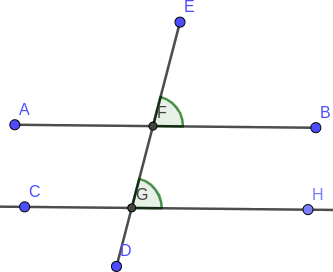
\includegraphics[width=\linewidth]{../images/ang_correspond01}
        % \begin{tikzpicture}
        %     \draw[fill=yellow] (0,0) -- (60:.75cm) arc (60:180:.75cm);
        %     \draw(120:0.4cm) node {$\alpha$};

        %     \draw[fill=green!30] (0,0) -- (right:.75cm) arc (0:60:.75cm);
        %     \draw(30:0.5cm) node {$\beta$};

        %     \begin{scope}[shift={(60:2cm)}]
        %         \draw[fill=green!30] (0,0) -- (180:.75cm) arc (180:240:.75cm);
        %         \draw (30:-0.5cm) node {$\gamma$};

        %         \draw[fill=yellow] (0,0) -- (240:.75cm) arc (240:360:.75cm);
        %         \draw (-60:0.4cm) node {$\delta$};
        %     \end{scope}

        %     \begin{scope}[thick]
        %         \draw (60:-1cm) node[fill=white] {$E$} -- (60:5cm) node[fill=white] {$F$};
        %         \draw[red]                   (-2,0) node[left] {$A$} -- (3,0)
        %         node[right]{$B$};
        %         \draw[blue,shift={(60:2cm)}] (-3,0) node[left] {$C$} -- (2,0)
        %         node[right]{$D$};

        %         \draw[shift={(60:1cm)},xshift=4cm]
        %         node [right,text width=6cm,rounded corners,fill=red!20,inner sep=1ex]
        %         {
        %             When we assume that $\color{red}AB$ and $\color{blue}CD$ are
        %             parallel, i.\,e., ${\color{red}AB} \mathbin{\|} \color{blue}CD$,
        %             then $\alpha = \delta$ and $\beta = \gamma$.
        %         };
        %     \end{scope}
        % \end{tikzpicture}
        \caption{}
        \label{fig:ang_correspond01}
    \end{figure}
\end{minipage}
